\documentclass{article}
\usepackage[utf8]{inputenc}
\usepackage[T1]{fontenc}
\usepackage{lmodern}
\usepackage{amsmath}
\usepackage{amssymb}
\usepackage{graphicx}
\usepackage{float}
\usepackage{array}
\usepackage{booktabs}

\title{Bioinformatika}
\author{Adrian Klimaševski}
\date{2025-11-11}

\begin{document}

\maketitle
\section{\textit{Lab1}}
\subsection{Atstumo funkcijos skaičiavimas}

Atstumo funkcija apskaičiuota taikant \textit{Euklido atstumo} formulę tarp normalizuotų kodonų ir dikodonų dažnių vektorių.

Yra 2 sekos: A ir B. Kiekvienai jų apskaičiuojami normalizuoti dažniai:

\[
f_{A,i} = \frac{n_{A,i}}{\sum_{j=1}^{N} n_{A,j}}, \quad 
f_{B,i} = \frac{n_{B,i}}{\sum_{j=1}^{N} n_{B,j}}
\]

kur:

\begin{itemize}
\item $n_{A,i}$ - kiek kartų kodonas arba dikodonas $i$ pasirodo sekoje A
\item $N = 4^3 = 64$ kodonų atveju arba $N = 4^6 =4096$ dikodonų atveju (4, nes \textit{A, T, G, C}, bei 3 ir 6, nes kodonų ir dikondonų ilgiai atitinkamai)
\item $f_{A,i}$ ir $f_{B,i}$ - atitinkamai normalizuoti dažniai
\end{itemize}

Ir tada tarp sekų A bei B apskaičiuojamas atstumas:

\[
d(A,B) = \sqrt{\sum_{i=1}^{N} (f_{A,i} - f_{B,i})^2}
\]

Gauta reikšmė $d(A,B)$ parodo, kiek skiriasi ir iš jų suformuojama matrica.


\subsection{Virusų sekų identifikavimas}

\begin{table}[H]
\centering
\caption{Virusų sekų atitikmenys}
\label{tab:virus_mapping}
\begin{tabular}{@{}lllll@{}}
\toprule
\textbf{Kodas} & \textbf{Tikras pavadinimas} & \textbf{Ilgis} & \textbf{Forward ORFs} & \textbf{Reverse ORFs} \\
\midrule
B1 & Lactococcus\_phage & 29305 & 28 & 35 \\
B2 & KM389305.1 & 28906 & 38 & 50 \\
B3 & NC\_028697.1 & 33900 & 41 & 43 \\
B4 & KC821626.1 & 28760 & 32 & 11 \\
M1 & coronavirus & 29903 & 15 & 29 \\
M2 & adenovirus & 34745 & 54 & 51 \\
M3 & U18337.1 & 29309 & 21 & 20 \\
M4 & herpesvirus & 25674 & 46 & 33 \\
\bottomrule
\end{tabular}
\end{table}

\subsection{Atstumų matricos}

\subsubsection{Kodonų atstumų matrica}

\begin{table}[H]
\centering
\caption{Kodonų dažnių atstumų matrica}
\label{tab:codon_matrix}
\small
\begin{tabular}{@{}lcccccccc@{}}
\toprule
 & \textbf{B1} & \textbf{B2} & \textbf{B3} & \textbf{B4} & \textbf{M1} & \textbf{M2} & \textbf{M3} & \textbf{M4} \\
\midrule
\textbf{B1} & 0.0000 & 0.0610 & 0.0446 & 0.0573 & 0.0581 & 0.0700 & 0.0516 & 0.0928 \\
\textbf{B2} & 0.0610 & 0.0000 & 0.0545 & 0.0919 & 0.0617 & 0.0394 & 0.0736 & 0.0534 \\
\textbf{B3} & 0.0446 & 0.0545 & 0.0000 & 0.0635 & 0.0579 & 0.0591 & 0.0719 & 0.0836 \\
\textbf{B4} & 0.0573 & 0.0919 & 0.0635 & 0.0000 & 0.0782 & 0.0985 & 0.0672 & 0.1174 \\
\textbf{M1} & 0.0581 & 0.0617 & 0.0579 & 0.0782 & 0.0000 & 0.0628 & 0.0716 & 0.0849 \\
\textbf{M2} & 0.0700 & 0.0394 & 0.0591 & 0.0985 & 0.0628 & 0.0000 & 0.0899 & 0.0415 \\
\textbf{M3} & 0.0516 & 0.0736 & 0.0719 & 0.0672 & 0.0716 & 0.0899 & 0.0000 & 0.1038 \\
\textbf{M4} & 0.0928 & 0.0534 & 0.0836 & 0.1174 & 0.0849 & 0.0415 & 0.1038 & 0.0000 \\
\bottomrule
\end{tabular}
\end{table}

\subsubsection{Dikodonų atstumų matrica}

\begin{table}[H]
\centering
\caption{Dikodonų dažnių atstumų matrica}
\label{tab:dicodon_matrix}
\small
\begin{tabular}{@{}lcccccccc@{}}
\toprule
 & \textbf{B1} & \textbf{B2} & \textbf{B3} & \textbf{B4} & \textbf{M1} & \textbf{M2} & \textbf{M3} & \textbf{M4} \\
\midrule
\textbf{B1} & 0.0000 & 0.0198 & 0.0179 & 0.0228 & 0.0202 & 0.0198 & 0.0194 & 0.0235 \\
\textbf{B2} & 0.0198 & 0.0000 & 0.0189 & 0.0271 & 0.0203 & 0.0164 & 0.0219 & 0.0185 \\
\textbf{B3} & 0.0179 & 0.0189 & 0.0000 & 0.0228 & 0.0196 & 0.0185 & 0.0218 & 0.0222 \\
\textbf{B4} & 0.0228 & 0.0271 & 0.0228 & 0.0000 & 0.0250 & 0.0265 & 0.0237 & 0.0297 \\
\textbf{M1} & 0.0202 & 0.0203 & 0.0196 & 0.0250 & 0.0000 & 0.0193 & 0.0226 & 0.0228 \\
\textbf{M2} & 0.0198 & 0.0164 & 0.0185 & 0.0265 & 0.0193 & 0.0000 & 0.0229 & 0.0165 \\
\textbf{M3} & 0.0194 & 0.0219 & 0.0218 & 0.0237 & 0.0226 & 0.0229 & 0.0000 & 0.0252 \\
\textbf{M4} & 0.0235 & 0.0185 & 0.0222 & 0.0297 & 0.0228 & 0.0165 & 0.0252 & 0.0000 \\
\bottomrule
\end{tabular}
\end{table}

\subsection{Matricų analizė}

\subsubsection{Artimiausios ir tolimiausios poros}

\begin{table}[H]
\centering
\caption{Artimiausių ir tolimiausių virusų porų palyginimas}
\label{tab:distance_comparison}
\begin{tabular}{@{}llcc@{}}
\toprule
\textbf{Poros tipas} & \textbf{Virusų pora} & \textbf{Kodonų atstumas} & \textbf{Dikodonų atstumas} \\
\midrule
\textbf{Artimiausios} & B2-M2 & 0.0394 & 0.0164 \\
 & B1-B3 & 0.0446 & 0.0179 \\
 & M2-M4 & 0.0415 & 0.0165 \\
\midrule
\textbf{Tolimiausios} & B4-M4 & 0.1174 & 0.0297 \\
 & B4-M2 & 0.0985 & 0.0265 \\
 & B4-M1 & 0.0782 & 0.0250 \\
\bottomrule
\end{tabular}
\end{table}

\subsection*{Stebimi modeliai}

\begin{itemize}
\item Dikodonų atstumai yra žymiai mažesni (3-4 kartus) nei kodonų atstumai
\item Artimiausios poros išlieka panašios abiejuose lygmenyse: 
  \begin{itemize}
  \item B2(KM389305.1) - M2(adenovirus)
  \item B1(Lactococcus\_phage) - B3(NC\_028697.1) 
  \item M2(adenovirus) - M4(herpesvirus)
  \end{itemize}
\item Tolimiausios poros visada apima B4(KC821626.1) virusą
\end{itemize}



\subsection{Filogenetiniai medžiai}

\subsubsection{Kodonų medis}
\begin{figure}[H]
\centering
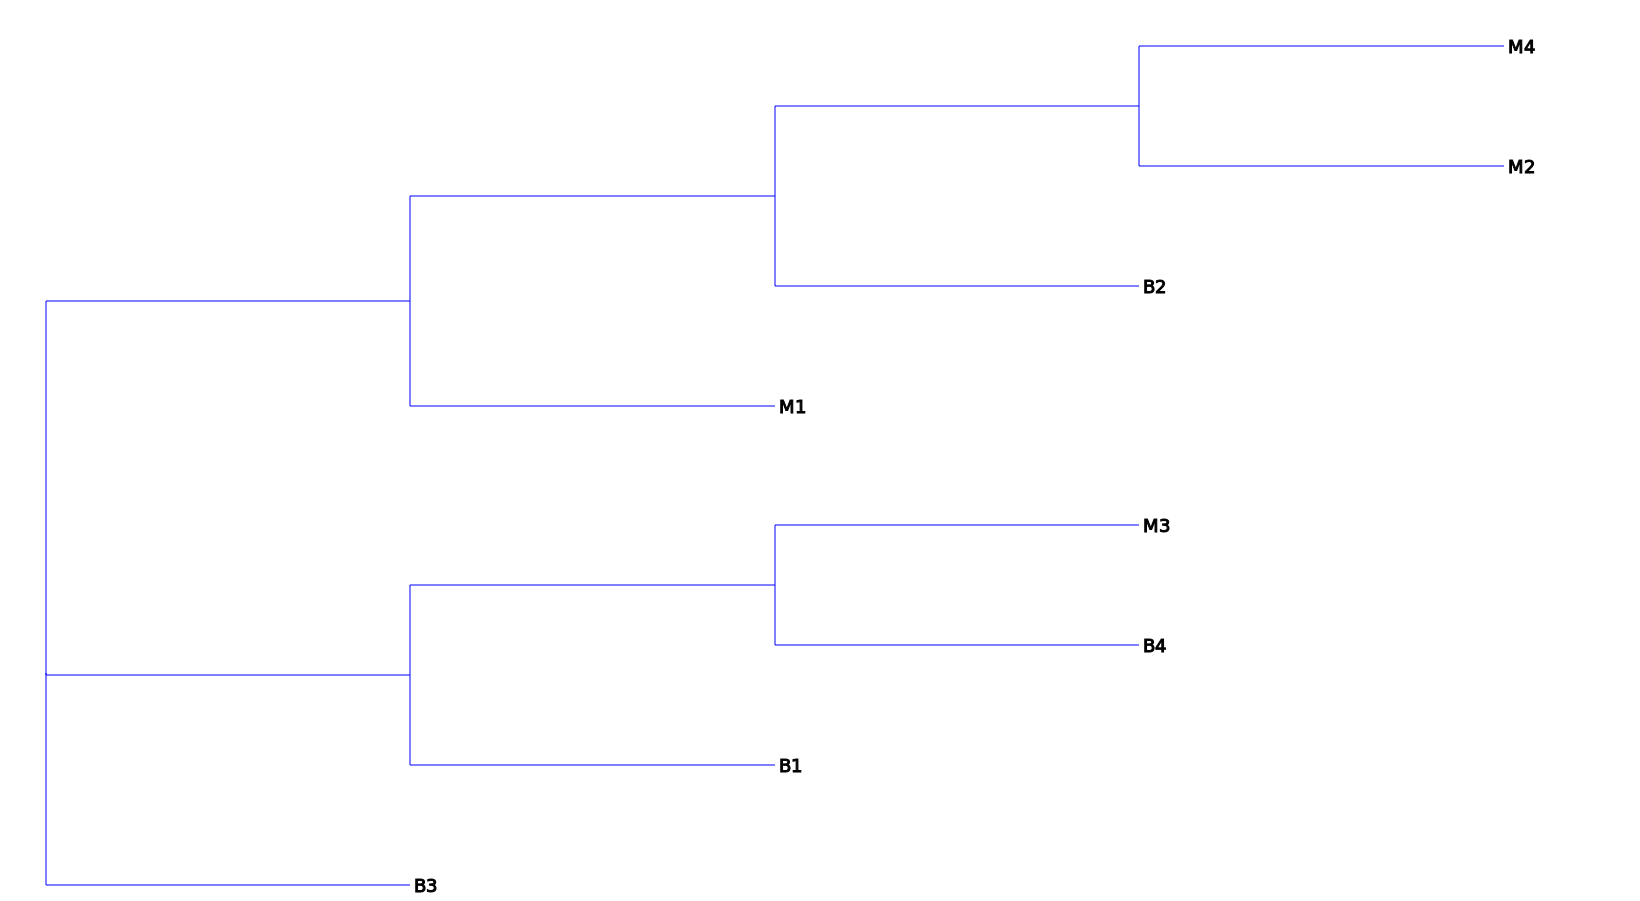
\includegraphics[width=1.2\textwidth]{codon_tree.png}
\caption{Filogenetinis medis pagal kodonų dažnius}
\label{fig:codon_tree}
\end{figure}

\subsubsection{Dikodonų medis}
\begin{figure}[H]
\centering
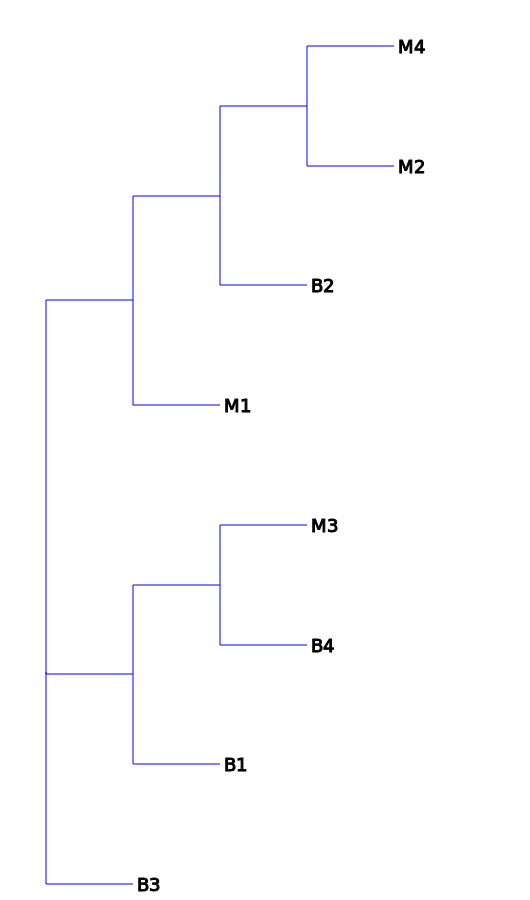
\includegraphics[width=0.8\textwidth]{dicodon_tree.png}
\caption{Filogenetinis medis pagal dikodonų dažnius}
\label{fig:dicodon_tree}
\end{figure}


\subsection{Extra informacija}

\subsubsection{Kodonų medžio rezultatai}


\begin{verbatim}
(M1:0.2662,(B3:0.1994,(B1:0.1687,(B4:0.3729,M3:0.2990):0.0401):0.0937):0.0479,
(B2:0.1433,(M2:0.1107,M4:0.3044):0.1131):0.1704);
\end{verbatim}

\begin{itemize}
\item Weight matrix: $W=1/D^{0.000000}$
\item Tree reconstruction method: Weighted least-squares method MW (global optimization)
\end{itemize}

\textbf{Tree Metric (Additive Distance) Matrix:}
\begin{verbatim}
B1    0.000000 0.062391 0.046181 0.058174 0.057651 0.070446 0.050778 0.089810 
B2    0.062391 0.000000 0.056091 0.086822 0.057988 0.036709 0.079426 0.056073 
B3    0.046181 0.056091 0.000000 0.070613 0.051352 0.064147 0.063217 0.083511 
B4    0.058174 0.086822 0.070613 0.000000 0.082083 0.094878 0.067192 0.114242 
M1    0.057651 0.057988 0.051352 0.082083 0.000000 0.066043 0.074687 0.085407 
M2    0.070446 0.036709 0.064147 0.094878 0.066043 0.000000 0.087482 0.041510 
M3    0.050778 0.079426 0.063217 0.067192 0.074687 0.087482 0.000000 0.106846 
M4    0.089810 0.056073 0.083511 0.114242 0.085407 0.041510 0.106846 0.000000 
\end{verbatim}

\textbf{Statistics:}
\begin{itemize}
\item Least-squares coefficient $\sum_{i<j}(Dij-ADij)^2 = 0.0003735881$
\item Average absolute difference $\sum_{i<j}|Dij-ADij|/(n(n-1)/2) = 0.0028781161$
\item Maximum absolute difference $\max_{i,j}|Dij-ADij| = 0.0086831878$
\item Total length of the tree $L = 0.2329761219$
\end{itemize}

\textbf{Tree Edge Lengths:}
\begin{verbatim}
9--4   0.037294
10--9  0.004009
9--7   0.029898
11--3  0.019941
12--5  0.026624
13--2  0.014327
14--6  0.011073
1--10  0.016871
10--11 0.009369
11--12 0.004787
12--13 0.017037
13--14 0.011309
14--8  0.030437
\end{verbatim}

\subsubsection{Dikodonų medžio rezultatai}

\begin{verbatim}
(M1:0.9825,(B3:0.8475,(B1:0.8395,(B4:1.3523,M3:1.0172):0.0858):0.1091):0.0638,
(B2:0.8005,(M2:0.6709,M4:0.9792):0.1194):0.2010);
\end{verbatim}

\begin{itemize}
\item Weight matrix: $W=1/D^{0.000000}$
\item Tree reconstruction method: Weighted least-squares method MW (global optimization)
\end{itemize}

\textbf{Tree Metric (Additive Distance) Matrix:}
\begin{verbatim}
B1    0.000000 0.020138 0.017960 0.022775 0.019948 0.020036 0.019424 0.023119 
B2    0.020138 0.000000 0.019128 0.026124 0.019840 0.015908 0.022773 0.018991 
B3    0.017960 0.019128 0.000000 0.023946 0.018937 0.019026 0.020595 0.022109 
B4    0.022775 0.026124 0.023946 0.000000 0.025933 0.026022 0.023695 0.029105 
M1    0.019948 0.019840 0.018937 0.025933 0.000000 0.019738 0.022583 0.022821 
M2    0.020036 0.015908 0.019026 0.026022 0.019738 0.000000 0.022671 0.016502 
M3    0.019424 0.022773 0.020595 0.023695 0.022583 0.022671 0.000000 0.025754 
M4    0.023119 0.018991 0.022109 0.029105 0.022821 0.016502 0.025754 0.000000 
\end{verbatim}

\textbf{Statistics:}
\begin{itemize}
\item Least-squares coefficient $\sum_{i<j}(Dij-ADij)^2 = 0.0000083402$
\item Average absolute difference $\sum_{i<j}|Dij-ADij|/(n(n-1)/2) = 0.0004192914$
\item Maximum absolute difference $\max_{i,j}|Dij-ADij| = 0.0012051365$
\item Total length of the tree $L = 0.0806854125$
\end{itemize}

\textbf{Tree Edge Lengths:}
\begin{verbatim}
9--7   0.010172
10--9  0.000858
9--4   0.013523
11--3  0.008475
12--5  0.009825
13--2  0.008005
14--6  0.006709
1--10  0.008395
10--11 0.001091
11--12 0.000638
12--13 0.002010
13--14 0.001194
14--8  0.009792
\end{verbatim}



\subsection{Rezultatai ir išvados}

\subsubsection*{Ar skiriasi kodonų ir dikodonų dažnis tarp žinduolių ir bakterijų virusų?}

\textbf{Atsakymas:} Taip, skiriasi.

\subsubsection*{Kaip klasterizuojasi virusai?}

\textbf{Atsakymas:} Abiejuose medžiuose grupuojasi panašiai.

\textbf{Artimiausios poros}: 
\begin{itemize}
\item B1(Lactococcus\_phage) - B3(NC\_028697.1) (atstumas: 0.0462 kodonų, 0.0180 dikodonų)
\item M2(adenovirus) - M4(herpesvirus) (atstumas: 0.0415 kodonų, 0.0165 dikodonų)
\end{itemize}

\textbf{Kiti pastebėjimai}:
\begin{itemize}
\item Stipriausias klasteris: B1(Lactococcus\_phage) - B3(NC\_028697.1) - B4(KC821626.1) su M3(U18337.1)
\item M3(U18337.1) virusas nuolat grupuojasi su bakteriniais virusais
\item Neaiški atskirtis tarp bakterinių ir žinduolių virusų
\end{itemize}

\subsubsection*{Kuris virusas labiausiai išsiskyrė?}

\textbf{Atsakymas:} išsiskyrė labiausiai M3(U18337.1) virusas

\begin{itemize}
\item Abiejuose medžiuose yra artimesnis bakteriniams virusams B4(KC821626.1)
\item Atstumas nuo kitų žinduolių virusų:
  \begin{itemize}
  \item Iki M1(coronavirus): 0.0747 (kodonai), 0.0226 (dikodonai)
  \item Iki M2(adenovirus): 0.0875 (kodonai), 0.0227 (dikodonai)
  \item Iki M4(herpesvirus): 0.1068 (kodonai), 0.0258 (dikodonai)
  \end{itemize}
\item Atstumas iki B4(KC821626.1): 0.0672 (kodonai), 0.0237 (dikodonai)
\end{itemize}

\subsubsection*{Kokie kodonai/dikodonai labiausiai varijuoja?}

\begin{itemize}
\item \textbf{Didžiausi atstumai}: 
  \begin{itemize}
  \item B4(KC821626.1) - M4(herpesvirus)
  \item B4(KC821626.1) - M2(adenovirus) 
  \item B4(KC821626.1) - M1(coronavirus)
  \end{itemize}
\item \textbf{Mažiausi atstumai}:
  \begin{itemize}
  \item B1(Lactococcus\_phage) - B3(NC\_028697.1)
  \item M2(adenovirus) - M4(herpesvirus)
  \item B2(KM389305.1) - M2(adenovirus)
  \end{itemize}
\item B4(KC821626.1) virusas nuolat pasirodo tolimiausiose porose, rodant didžiausią kodonų/dikodonų naudojimo skirtumą
\end{itemize}

\end{document}